\documentclass{article}

% Add 'authorblk' package for affliation support
\usepackage{authblk}

% use package to control paper dimensions
\usepackage{geometry}
 \geometry{
		a4paper,
		% left=22mm,
		% right=22mm,
		top=20mm,
		bottom=20mm
	}

%use packahge to add graphics items
\usepackage{graphicx}

% set the title of the article
\title{
	Data Analytics - Assignment 2 \\
	\large Data Visualization Techniques on Bio-Informatics Data
	}

\author{R Mukesh (CED15I002), Kiran Robert (EVD15I007), Gajaraj G. (MPD15I011)}
\affil{IIITDM, Kancheepuram}

\date{October 10, 2018}

\begin{document}
\maketitle

	\begin{abstract}
		With the advent of the \textbf{Human Genome Project}, there has been an explosion of genomics data in the public domain. Data Visualization have become very crucial in comprehending and assimilating the growing pile of bio-informatics data. The article demonstrates some of the data visualization techniques on genomics data.
	\end{abstract}
	
	\section{Introduction}
		The DNA (Deoxyribonucleic Acid) is a molecule composed of two strands, each built from the four chemical building blocks (Cytosine[\textbf{C}], Guanine[\textbf{G}], Adenine[\textbf{A}] and Thymine[\textbf{T}]) called "bases". DNA sequencing is the process of determing the order of these "bases" in a DNA molecule.
		
		The DNA sequence dataset is a set strings composed of the four characters 'A', 'G', 'C' and 'T', each representing the four bases that make up a DNA molecule. The article makes use of one such DNA sequence dataset stored in the FASTA format.
	
	\section{Percentages of A, G, C, T in DNA sequences}
	
		The percentage of A,G,C,T and other unidentified bases in the DNA sequences are summarized and visually represented using the following charts.
		
		\subsection{Pie Chart}
			
			\begin{figure}[!htbp]
				\centering
				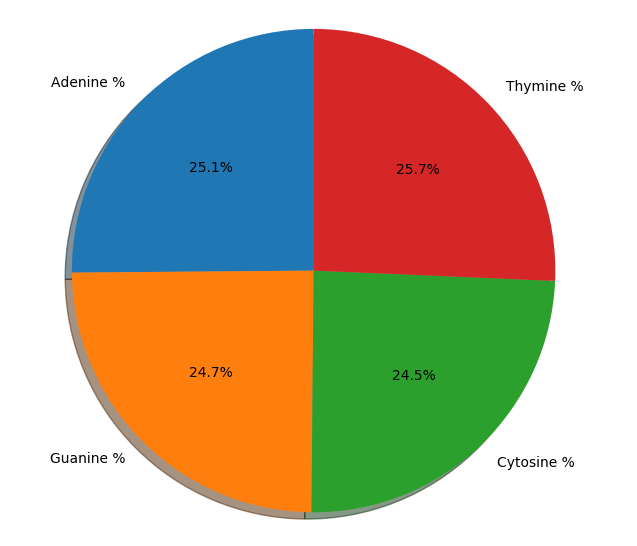
\includegraphics[scale=0.5]{charts/Figure_1}
				\caption{The average percentages of A,G,C,T across all DNA sequences.}
			\end{figure}
			
			\textbf{Inference:} The average percentage of A,G,C,T computed across all DNA sequences are approximately equal (about 25\%).
		
		\subsection{Box-Whisker Plot}
			
			\begin{figure}[!htbp]
				\centering
				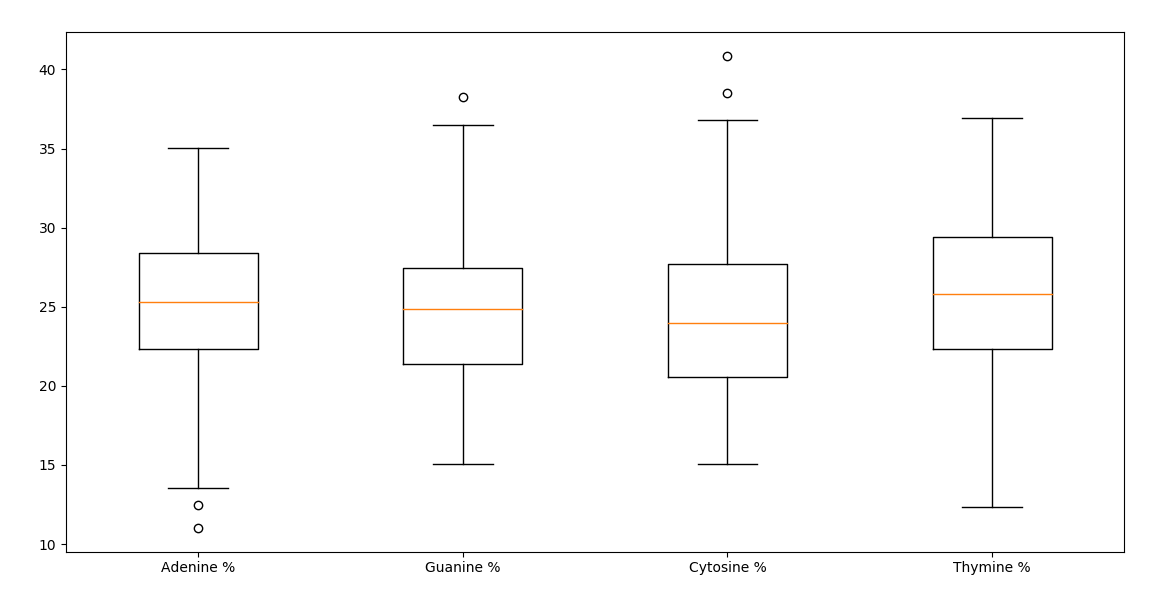
\includegraphics[scale=0.5]{charts/Figure_2}
				\caption{The Box-Whisker plot for percentages of each A,G,C,T for all DNA sequences.}
			\end{figure}
			
			
			\begin{itemize}\itemsep1pt
				\item [\textbf{Inferences:}]
				\item The percentages of each A,G,C,T have approximately the same distribution with minor variations. The meadian of the percentages of each A,G,C,T are approximately equal (about 25 \%).
				\item A few DNA sequences lie below the lower whisker or above the upper whisker indicating that they vary drastically from their respective distributions (outliers).
			\end{itemize}
			
		\subsection{Histogram}
			
			The histograms represent the count of DNA sequence with the different percentage ranges for 'A', 'G', 'C' and 'T'.
			\begin{figure}[!htbp]
				\centering
				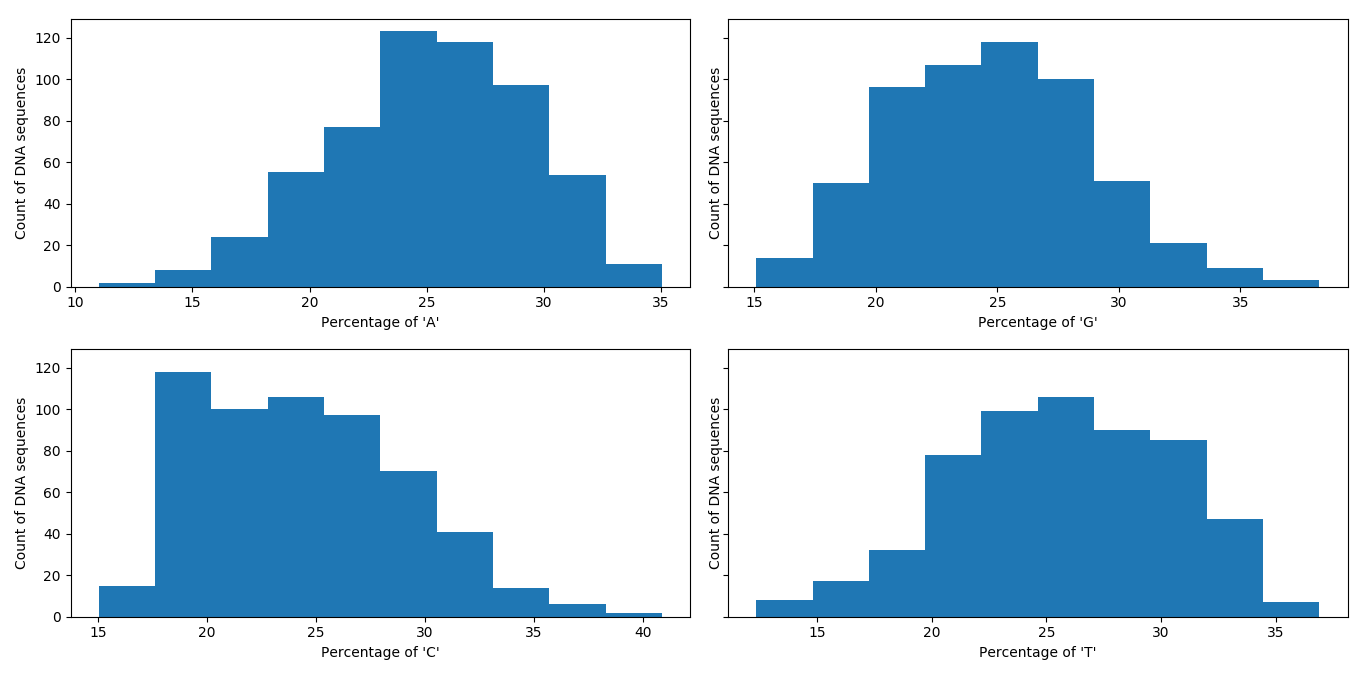
\includegraphics[scale=0.4]{charts/Figure_3}
				\caption{The histograms for the percentages of each A,G,C,T for all DNA sequences.}
			\end{figure}
			
			\textbf{Inference:} Majority of DNA sequences have percentages of 'A','G','C' and 'T' in ranges 20-30\%, 20-29\%, 18-28\% and 20-32\% respectively.
		
		\vspace{16pt}	
		
		\subsection{Violin Plot}
		
			\begin{figure}[!htbp]
				\centering
				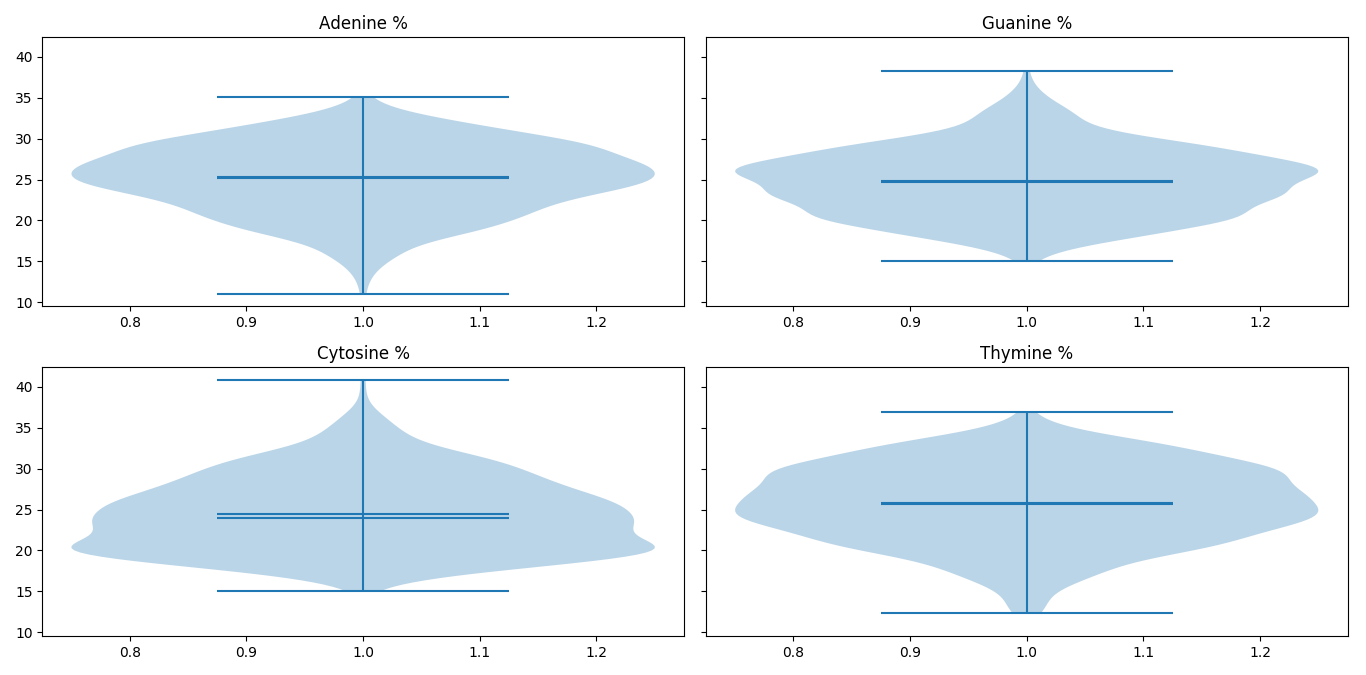
\includegraphics[scale=0.4]{charts/Figure_4}
				\caption{Violin plot for the percentages of each A,G,C,T for all DNA sequences.}
			\end{figure}
			
	\section{Number of occurrences of specific sub-sequences}
		The number of occurrences of the sub-sequences 'AC', 'CAG', 'TTAGGG' in the DNA sequences are summarized and visually represented using the following charts.
		
		\subsection{Bar Chart}
		
			\begin{figure}[!htbp]
				\centering
				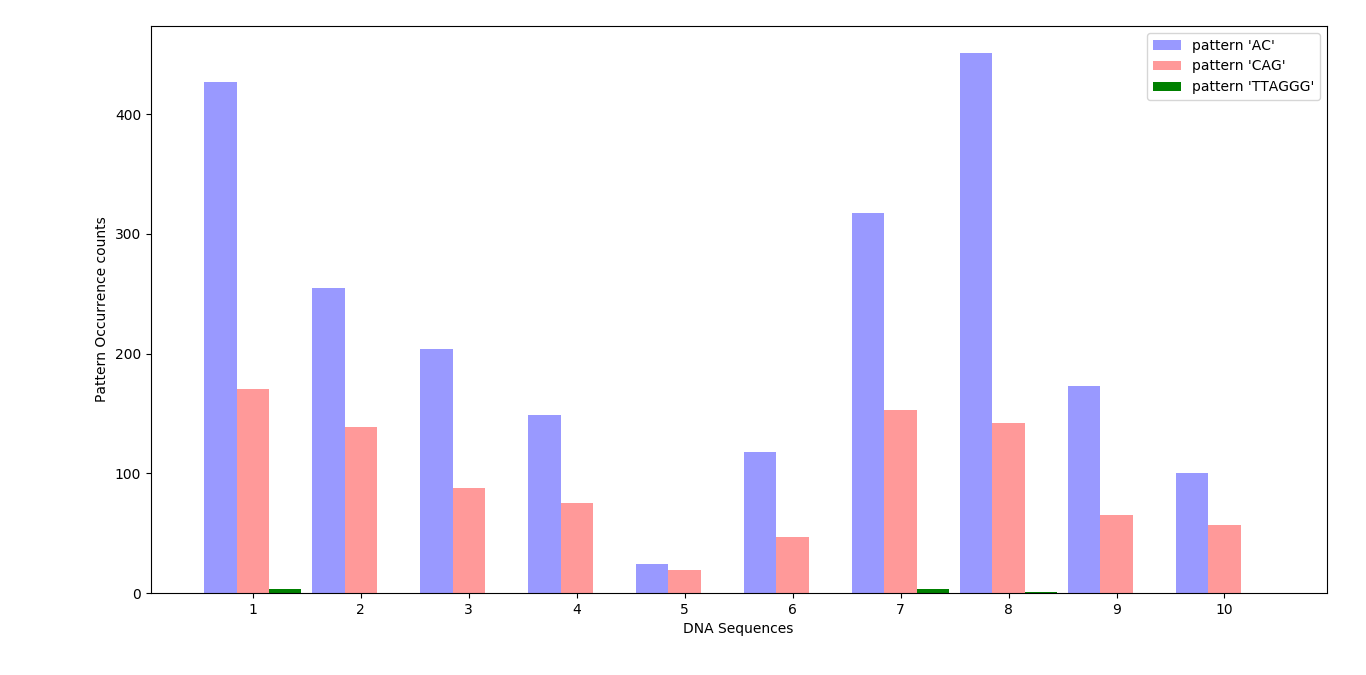
\includegraphics[scale=0.4]{charts/Figure_5}
				\caption{Bar chart for the count of different sub-sequence patterns in 10 randomly selected DNA sequences.}
			\end{figure}
			
			\textbf{Inference:} The number of occurrences of pattern 'AC' is much higher than number of occurrences of pattern 'CAG' for the DNA sequences. The number of occurrences of pattern 'TTAGGG' is negligible.
		
		\vspace{54pt}
		\subsection{Histogram}
		
			\begin{figure}[!htbp]
				\centering
				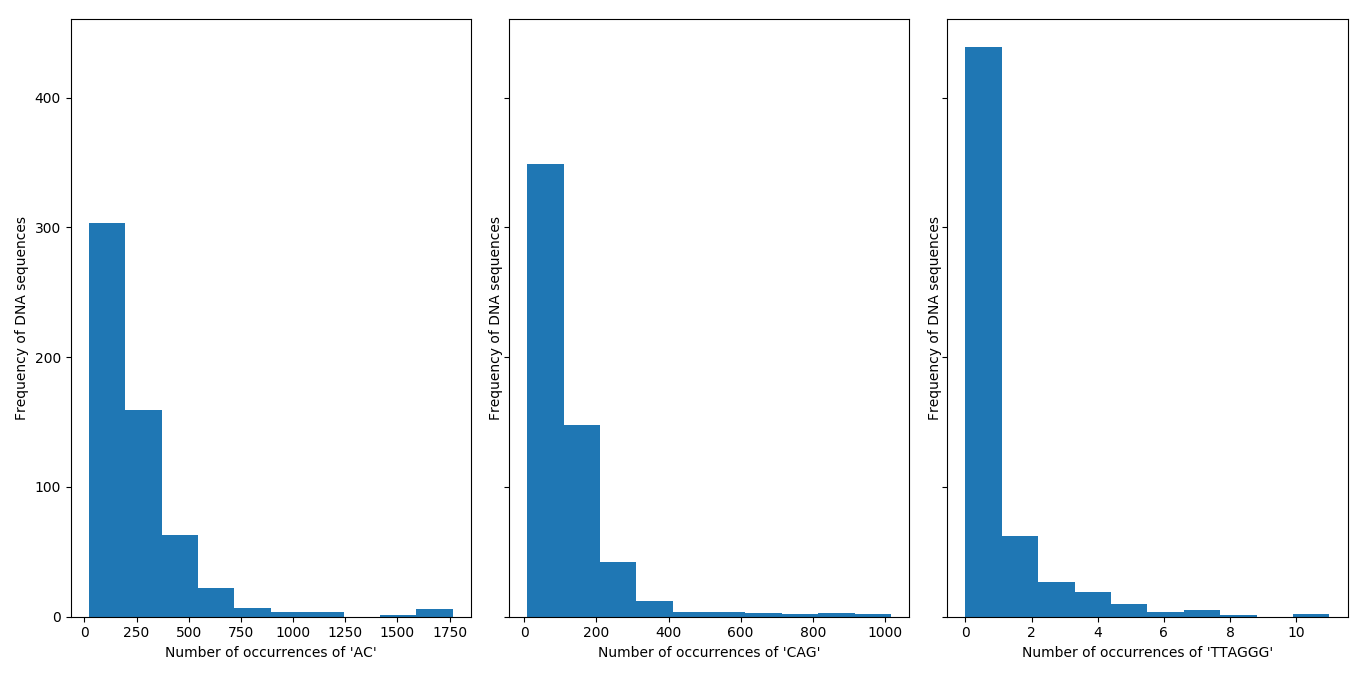
\includegraphics[scale=0.4]{charts/Figure_6}
				\caption{Histograms representing the frequency of DNA sequences for varying number of occurrences of the patterns 'AC', 'CAG' and 'TTAGGG' in the DNA sequence.}
			\end{figure}
			
			\begin{itemize}\itemsep1pt
				\item [\textbf{Inferences:}]
				\item About 300 DNA sequences have the number of occurrence of pattern 'AC' in range 0 to 170. About 350 DNA sequences have number of occurrences of pattern 'CAG' in range 0 to 100. About 440 DNA sequences have number of occurrences of pattern 'TTAGGG' in range 0 to 1.
				\item Negligible number of DNA sequences have number of occurrences of pattern 'AC' above 700, number of occurrences of pattern 'CAG' above 400 and number of occurrences of pattern 'TTAGG' above 5.
			\end{itemize}
		
				\subsection{Box-Whisker Plot}
			
			\begin{figure}[!htbp]
				\centering
				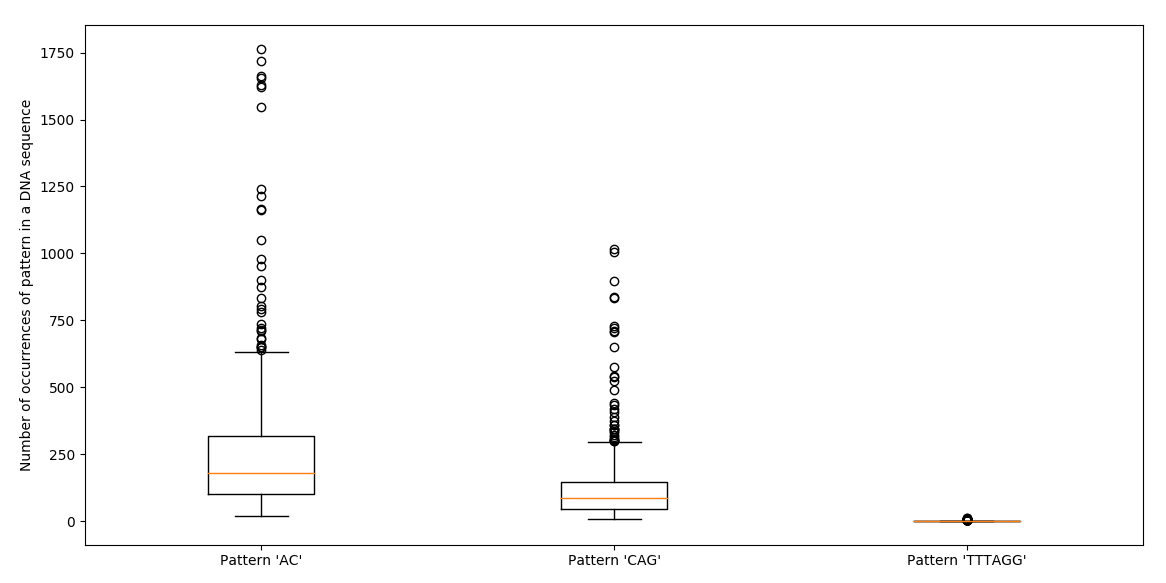
\includegraphics[scale=0.4]{charts/Figure_7}
				\caption{Box-Whisker plot for the number of occurrences of pattern 'AC', 'CAG', 'TTAGGG' for each DNA sequence.}
			\end{figure}
			
			\begin{itemize}\itemsep1pt
				\item [\textbf{Inferences:}]
				\item The distribution of number of occurrence of pattern 'AC' has more variation than that for 'CAG'. The distribution of number of occurrences of pattern 'TTAGGG' has least variation.
				\item The distribution number of occurrences of pattern 'CAG' has lower median than distribution number of occurrences of pattern 'AC', which is inturn smaller than distribution number of occurrences of pattern 'TTAGGG'.
			\end{itemize}

		\subsection{Violin Plot}
		
			\begin{figure}[!htbp]
				\centering
				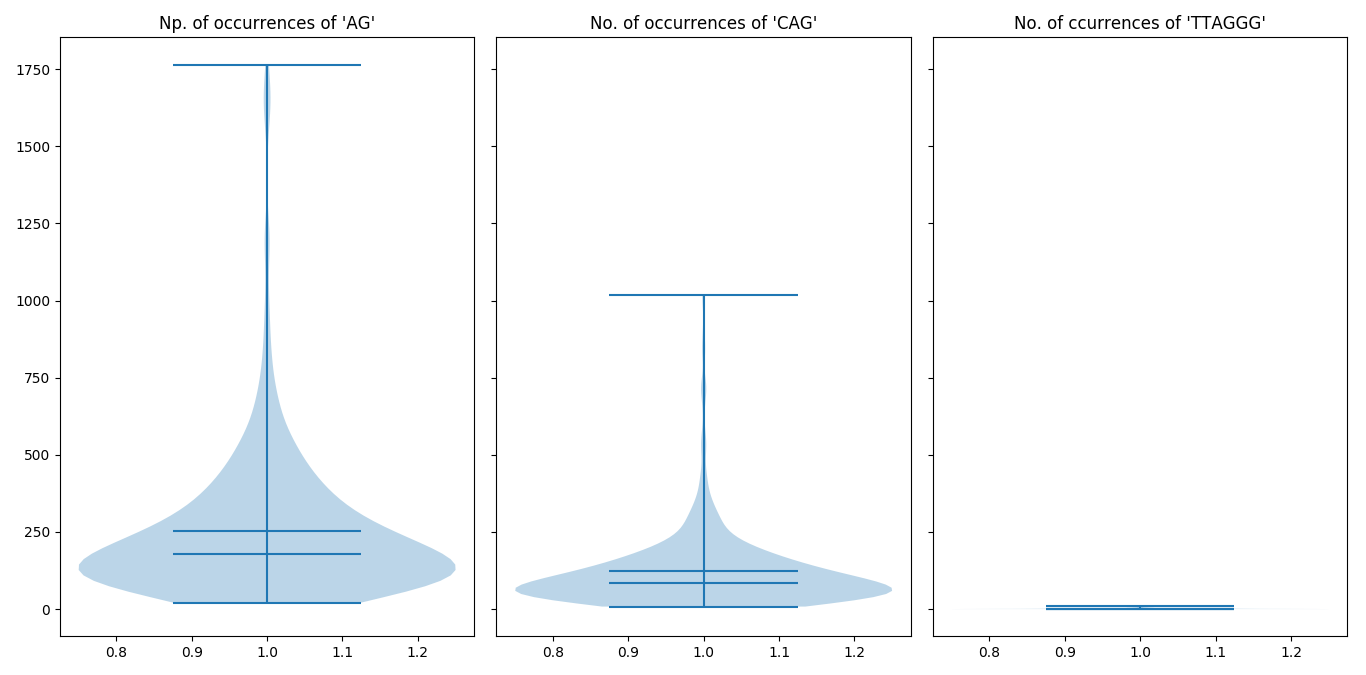
\includegraphics[scale=0.4]{charts/Figure_8}
				\caption{Violin plot for the number of occurrences of pattern 'AC', 'CAG', 'TTAGGG' for each DNA sequence.}
			\end{figure}
		
		\subsection{Scatter Plot}
			
			The scatter plot seeks to find the correlation(if any) between the values of number of occurrences of pattern 'AC' and 'CAG' for the DNA sequences.
			
			\begin{figure}[!htbp]
				\centering
				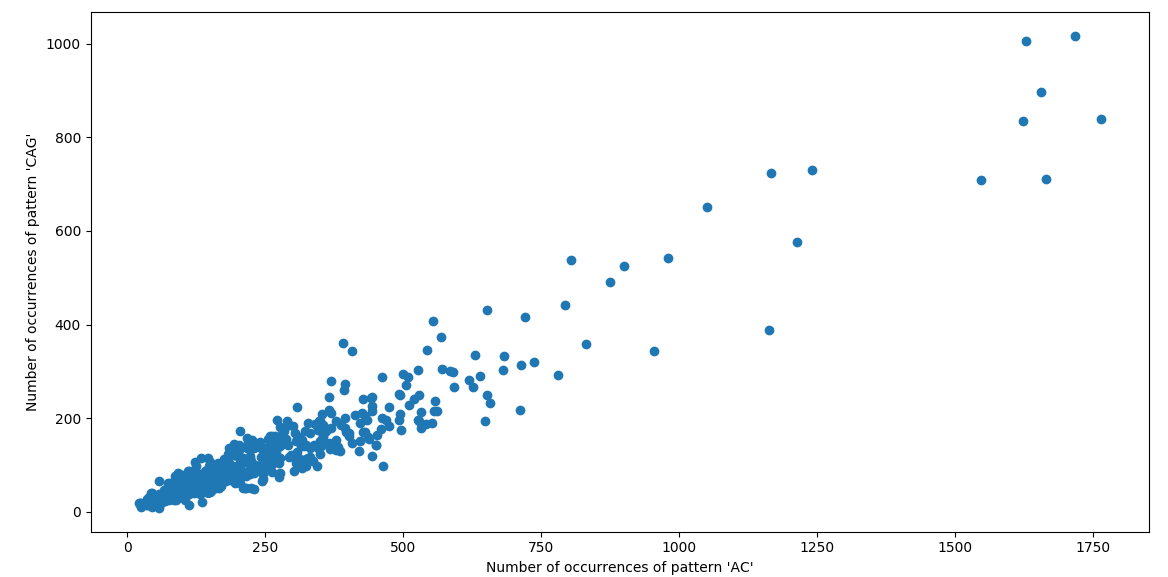
\includegraphics[scale=0.48]{charts/Figure_9}
				\caption{Scatter plot between the number of occurrences of pattern 'AC' and 'CAG', 'TTAGGG' for the DNA sequences.}
			\end{figure}
		
	\section{Length of DNA sequence}
		The length of the DNA sequences are summarized and visually represented using the following charts.
			
			\vspace{51pt}
			\subsection{Box-Whisker Plot}
				\begin{figure}[!htbp]
					\centering
					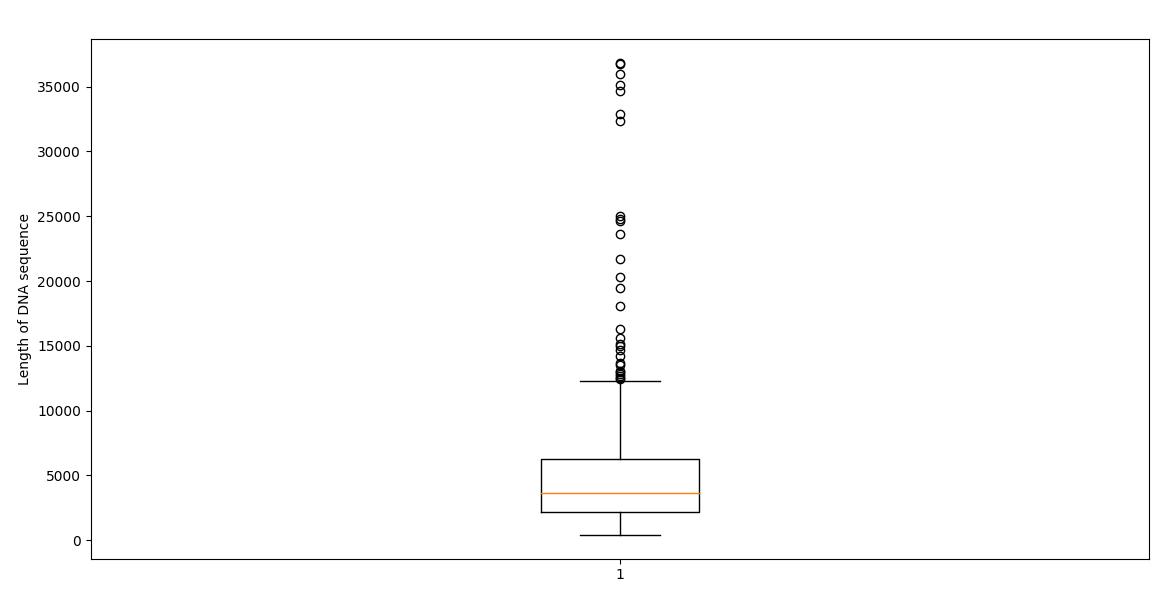
\includegraphics[scale=0.48]{charts/Figure_13}
					\caption{Box-Whisker plot representing the lengths of the DNA sequences.}
				\end{figure}
				
				\begin{itemize}
					\item[\textbf{Inference:}]
					\item The distribution of length of all the DNA sequences has median of approximately 2500. 
					\item The DNA sequences that lie above the upper whisker have lengths much higher than the distribution median (outliers).
				\end{itemize}
			
			\subsection{Histogram}
				\begin{figure}[!htbp]
					\centering
					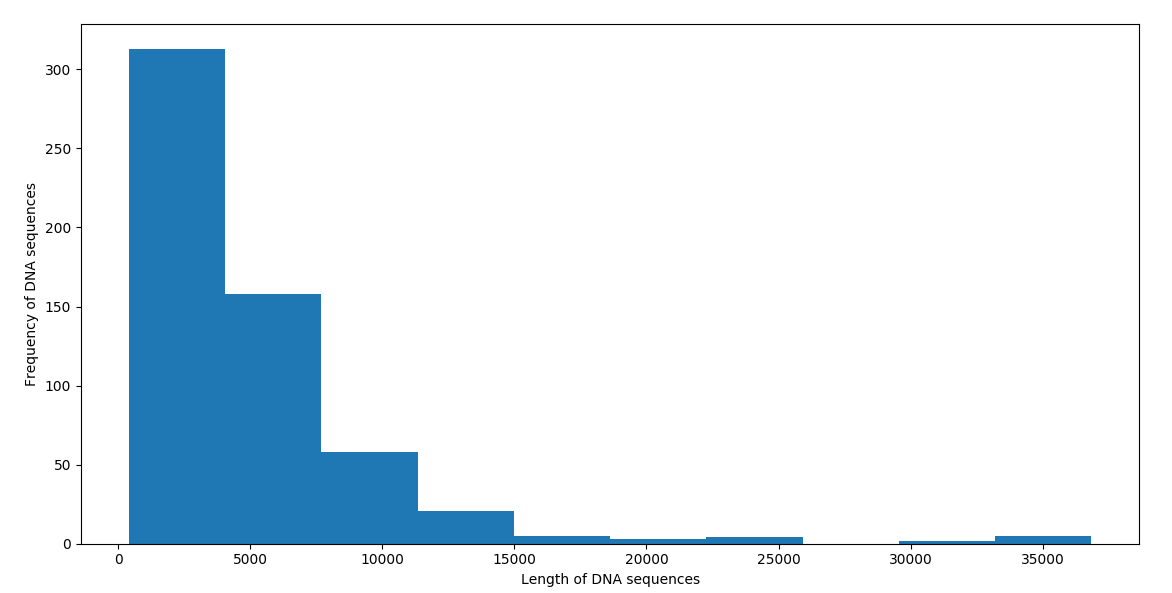
\includegraphics[scale=0.48]{charts/Figure_14}
					\caption{Histogram plot representing the frequency of DNA sequences with various lengths.}
				\end{figure}
			
			\vspace{83pt}
			\subsection{Violin Plot}
				\begin{figure}[!htbp]
					\centering
					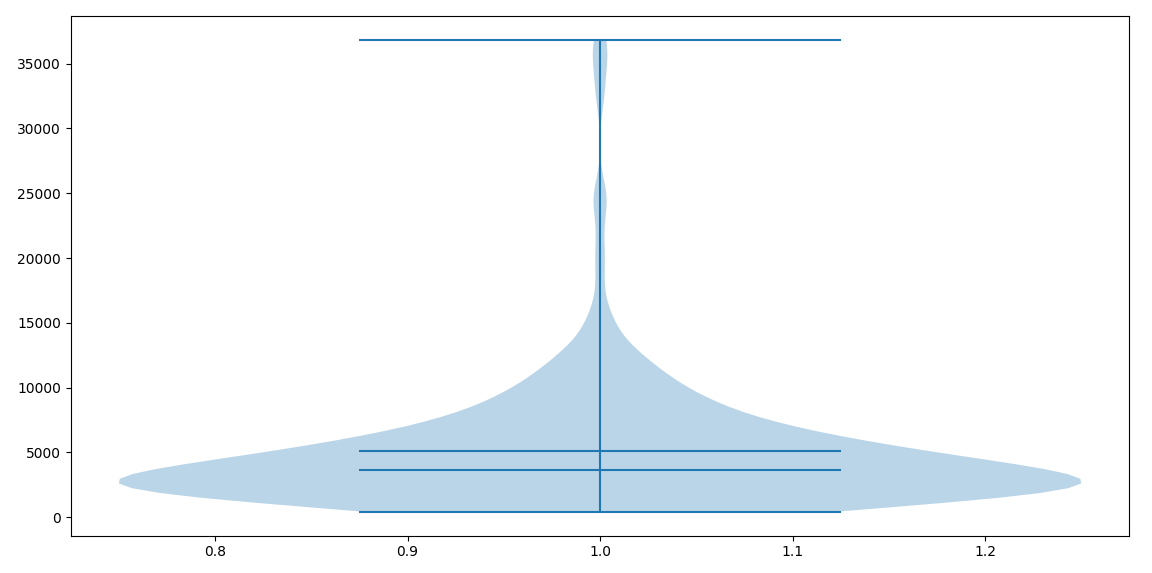
\includegraphics[scale=0.48]{charts/Figure_15}
					\caption{Violin plot for the lengths of the DNA sequences.}
				\end{figure}
				
\end{document}